% Created by tikzDevice version 0.10.1 on 2018-01-25 15:36:29
% !TEX encoding = UTF-8 Unicode
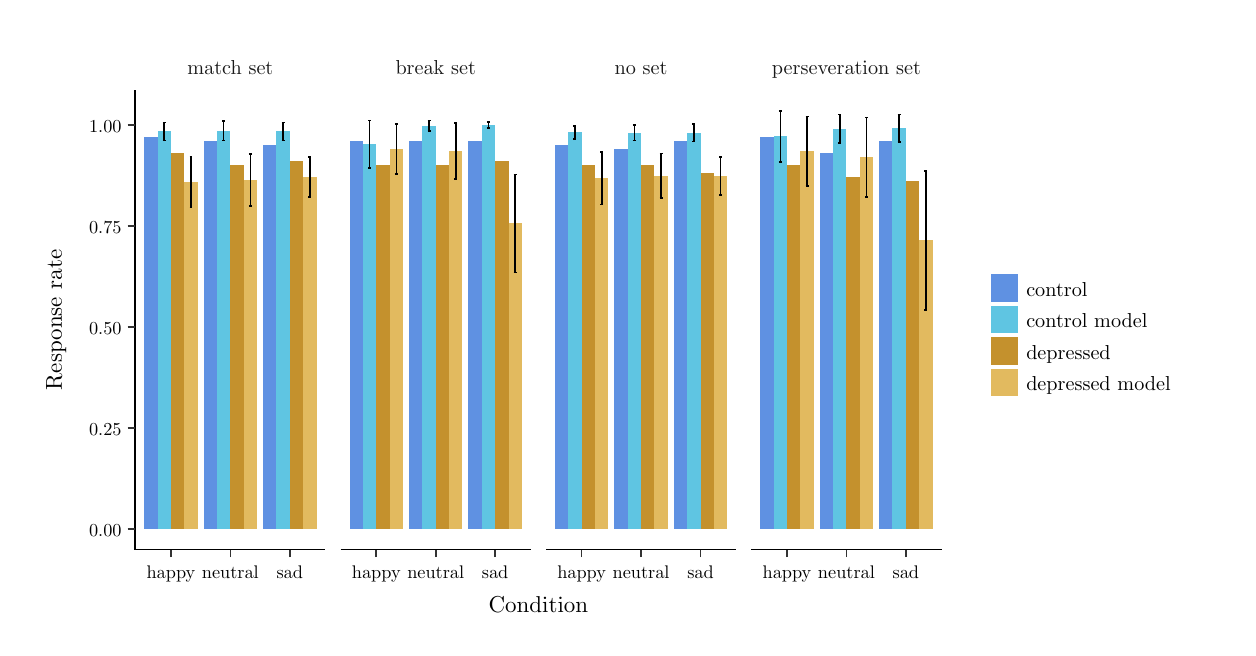
\begin{tikzpicture}[x=1pt,y=1pt]
\definecolor{fillColor}{RGB}{255,255,255}
\path[use as bounding box,fill=fillColor,fill opacity=0.00] (0,0) rectangle (433.62,216.81);
\begin{scope}
\path[clip] (  0.00,  0.00) rectangle (433.62,216.81);
\definecolor{drawColor}{RGB}{255,255,255}
\definecolor{fillColor}{RGB}{255,255,255}

\path[draw=drawColor,line width= 0.6pt,line join=round,line cap=round,fill=fillColor] (  0.00,  0.00) rectangle (433.62,216.81);
\end{scope}
\begin{scope}
\path[clip] ( 38.88, 28.22) rectangle (107.59,194.25);
\definecolor{fillColor}{RGB}{255,255,255}

\path[fill=fillColor] ( 38.88, 28.22) rectangle (107.59,194.25);
\definecolor{fillColor}{RGB}{226,186,95}

\path[fill=fillColor] ( 56.60, 35.77) rectangle ( 61.43,161.02);
\definecolor{fillColor}{RGB}{196,145,45}

\path[fill=fillColor] ( 51.77, 35.77) rectangle ( 56.60,171.47);
\definecolor{fillColor}{RGB}{95,197,226}

\path[fill=fillColor] ( 46.94, 35.77) rectangle ( 51.77,179.30);
\definecolor{fillColor}{RGB}{95,145,226}

\path[fill=fillColor] ( 42.11, 35.77) rectangle ( 46.94,177.30);
\definecolor{fillColor}{RGB}{226,186,95}

\path[fill=fillColor] ( 78.07, 35.77) rectangle ( 82.90,161.80);
\definecolor{fillColor}{RGB}{196,145,45}

\path[fill=fillColor] ( 73.24, 35.77) rectangle ( 78.07,167.09);
\definecolor{fillColor}{RGB}{95,197,226}

\path[fill=fillColor] ( 68.41, 35.77) rectangle ( 73.24,179.57);
\definecolor{fillColor}{RGB}{95,145,226}

\path[fill=fillColor] ( 63.58, 35.77) rectangle ( 68.41,175.84);
\definecolor{fillColor}{RGB}{226,186,95}

\path[fill=fillColor] ( 99.54, 35.77) rectangle (104.37,162.79);
\definecolor{fillColor}{RGB}{196,145,45}

\path[fill=fillColor] ( 94.71, 35.77) rectangle ( 99.54,168.55);
\definecolor{fillColor}{RGB}{95,197,226}

\path[fill=fillColor] ( 89.88, 35.77) rectangle ( 94.71,179.29);
\definecolor{fillColor}{RGB}{95,145,226}

\path[fill=fillColor] ( 85.05, 35.77) rectangle ( 89.88,174.39);
\definecolor{drawColor}{RGB}{0,0,0}

\path[draw=drawColor,line width= 0.6pt,line join=round] ( 58.48,170.16) --
	( 59.55,170.16);

\path[draw=drawColor,line width= 0.6pt,line join=round] ( 59.01,170.16) --
	( 59.01,151.87);

\path[draw=drawColor,line width= 0.6pt,line join=round] ( 58.48,151.87) --
	( 59.55,151.87);

\path[draw=drawColor,line width= 0.6pt,line join=round] ( 48.81,182.56) --
	( 49.89,182.56);

\path[draw=drawColor,line width= 0.6pt,line join=round] ( 49.35,182.56) --
	( 49.35,176.04);

\path[draw=drawColor,line width= 0.6pt,line join=round] ( 48.81,176.04) --
	( 49.89,176.04);

\path[draw=drawColor,line width= 0.6pt,line join=round] ( 79.95,171.17) --
	( 81.02,171.17);

\path[draw=drawColor,line width= 0.6pt,line join=round] ( 80.49,171.17) --
	( 80.49,152.43);

\path[draw=drawColor,line width= 0.6pt,line join=round] ( 79.95,152.43) --
	( 81.02,152.43);

\path[draw=drawColor,line width= 0.6pt,line join=round] ( 70.29,183.12) --
	( 71.36,183.12);

\path[draw=drawColor,line width= 0.6pt,line join=round] ( 70.82,183.12) --
	( 70.82,176.02);

\path[draw=drawColor,line width= 0.6pt,line join=round] ( 70.29,176.02) --
	( 71.36,176.02);

\path[draw=drawColor,line width= 0.6pt,line join=round] (101.42,170.00) --
	(102.49,170.00);

\path[draw=drawColor,line width= 0.6pt,line join=round] (101.96,170.00) --
	(101.96,155.57);

\path[draw=drawColor,line width= 0.6pt,line join=round] (101.42,155.57) --
	(102.49,155.57);

\path[draw=drawColor,line width= 0.6pt,line join=round] ( 91.76,182.58) --
	( 92.83,182.58);

\path[draw=drawColor,line width= 0.6pt,line join=round] ( 92.29,182.58) --
	( 92.29,176.00);

\path[draw=drawColor,line width= 0.6pt,line join=round] ( 91.76,176.00) --
	( 92.83,176.00);
\end{scope}
\begin{scope}
\path[clip] (113.09, 28.22) rectangle (181.80,194.25);
\definecolor{fillColor}{RGB}{255,255,255}

\path[fill=fillColor] (113.09, 28.22) rectangle (181.80,194.25);
\definecolor{fillColor}{RGB}{226,186,95}

\path[fill=fillColor] (130.81, 35.77) rectangle (135.64,172.92);
\definecolor{fillColor}{RGB}{196,145,45}

\path[fill=fillColor] (125.98, 35.77) rectangle (130.81,167.09);
\definecolor{fillColor}{RGB}{95,197,226}

\path[fill=fillColor] (121.14, 35.77) rectangle (125.98,174.67);
\definecolor{fillColor}{RGB}{95,145,226}

\path[fill=fillColor] (116.31, 35.77) rectangle (121.14,175.84);
\definecolor{fillColor}{RGB}{226,186,95}

\path[fill=fillColor] (152.28, 35.77) rectangle (157.11,172.22);
\definecolor{fillColor}{RGB}{196,145,45}

\path[fill=fillColor] (147.45, 35.77) rectangle (152.28,167.09);
\definecolor{fillColor}{RGB}{95,197,226}

\path[fill=fillColor] (142.62, 35.77) rectangle (147.45,181.42);
\definecolor{fillColor}{RGB}{95,145,226}

\path[fill=fillColor] (137.78, 35.77) rectangle (142.62,175.84);
\definecolor{fillColor}{RGB}{226,186,95}

\path[fill=fillColor] (173.75, 35.77) rectangle (178.58,146.05);
\definecolor{fillColor}{RGB}{196,145,45}

\path[fill=fillColor] (168.92, 35.77) rectangle (173.75,168.55);
\definecolor{fillColor}{RGB}{95,197,226}

\path[fill=fillColor] (164.09, 35.77) rectangle (168.92,181.53);
\definecolor{fillColor}{RGB}{95,145,226}

\path[fill=fillColor] (159.26, 35.77) rectangle (164.09,175.84);
\definecolor{drawColor}{RGB}{0,0,0}

\path[draw=drawColor,line width= 0.6pt,line join=round] (132.69,181.90) --
	(133.76,181.90);

\path[draw=drawColor,line width= 0.6pt,line join=round] (133.22,181.90) --
	(133.22,163.94);

\path[draw=drawColor,line width= 0.6pt,line join=round] (132.69,163.94) --
	(133.76,163.94);

\path[draw=drawColor,line width= 0.6pt,line join=round] (123.02,183.24) --
	(124.10,183.24);

\path[draw=drawColor,line width= 0.6pt,line join=round] (123.56,183.24) --
	(123.56,166.10);

\path[draw=drawColor,line width= 0.6pt,line join=round] (123.02,166.10) --
	(124.10,166.10);

\path[draw=drawColor,line width= 0.6pt,line join=round] (154.16,182.44) --
	(155.23,182.44);

\path[draw=drawColor,line width= 0.6pt,line join=round] (154.69,182.44) --
	(154.69,162.01);

\path[draw=drawColor,line width= 0.6pt,line join=round] (154.16,162.01) --
	(155.23,162.01);

\path[draw=drawColor,line width= 0.6pt,line join=round] (144.49,183.29) --
	(145.57,183.29);

\path[draw=drawColor,line width= 0.6pt,line join=round] (145.03,183.29) --
	(145.03,179.54);

\path[draw=drawColor,line width= 0.6pt,line join=round] (144.49,179.54) --
	(145.57,179.54);

\path[draw=drawColor,line width= 0.6pt,line join=round] (175.63,163.75) --
	(176.70,163.75);

\path[draw=drawColor,line width= 0.6pt,line join=round] (176.16,163.75) --
	(176.16,128.35);

\path[draw=drawColor,line width= 0.6pt,line join=round] (175.63,128.35) --
	(176.70,128.35);

\path[draw=drawColor,line width= 0.6pt,line join=round] (165.97,182.61) --
	(167.04,182.61);

\path[draw=drawColor,line width= 0.6pt,line join=round] (166.50,182.61) --
	(166.50,180.44);

\path[draw=drawColor,line width= 0.6pt,line join=round] (165.97,180.44) --
	(167.04,180.44);
\end{scope}
\begin{scope}
\path[clip] (187.30, 28.22) rectangle (256.01,194.25);
\definecolor{fillColor}{RGB}{255,255,255}

\path[fill=fillColor] (187.30, 28.22) rectangle (256.01,194.25);
\definecolor{fillColor}{RGB}{226,186,95}

\path[fill=fillColor] (205.01, 35.77) rectangle (209.85,162.40);
\definecolor{fillColor}{RGB}{196,145,45}

\path[fill=fillColor] (200.18, 35.77) rectangle (205.01,167.09);
\definecolor{fillColor}{RGB}{95,197,226}

\path[fill=fillColor] (195.35, 35.77) rectangle (200.18,179.02);
\definecolor{fillColor}{RGB}{95,145,226}

\path[fill=fillColor] (190.52, 35.77) rectangle (195.35,174.39);
\definecolor{fillColor}{RGB}{226,186,95}

\path[fill=fillColor] (226.49, 35.77) rectangle (231.32,163.28);
\definecolor{fillColor}{RGB}{196,145,45}

\path[fill=fillColor] (221.65, 35.77) rectangle (226.49,167.09);
\definecolor{fillColor}{RGB}{95,197,226}

\path[fill=fillColor] (216.82, 35.77) rectangle (221.65,178.86);
\definecolor{fillColor}{RGB}{95,145,226}

\path[fill=fillColor] (211.99, 35.77) rectangle (216.82,172.93);
\definecolor{fillColor}{RGB}{226,186,95}

\path[fill=fillColor] (247.96, 35.77) rectangle (252.79,163.16);
\definecolor{fillColor}{RGB}{196,145,45}

\path[fill=fillColor] (243.13, 35.77) rectangle (247.96,164.17);
\definecolor{fillColor}{RGB}{95,197,226}

\path[fill=fillColor] (238.29, 35.77) rectangle (243.13,178.90);
\definecolor{fillColor}{RGB}{95,145,226}

\path[fill=fillColor] (233.46, 35.77) rectangle (238.29,175.84);
\definecolor{drawColor}{RGB}{0,0,0}

\path[draw=drawColor,line width= 0.6pt,line join=round] (206.89,171.94) --
	(207.97,171.94);

\path[draw=drawColor,line width= 0.6pt,line join=round] (207.43,171.94) --
	(207.43,152.86);

\path[draw=drawColor,line width= 0.6pt,line join=round] (206.89,152.86) --
	(207.97,152.86);

\path[draw=drawColor,line width= 0.6pt,line join=round] (197.23,181.35) --
	(198.30,181.35);

\path[draw=drawColor,line width= 0.6pt,line join=round] (197.77,181.35) --
	(197.77,176.69);

\path[draw=drawColor,line width= 0.6pt,line join=round] (197.23,176.69) --
	(198.30,176.69);

\path[draw=drawColor,line width= 0.6pt,line join=round] (228.36,171.38) --
	(229.44,171.38);

\path[draw=drawColor,line width= 0.6pt,line join=round] (228.90,171.38) --
	(228.90,155.18);

\path[draw=drawColor,line width= 0.6pt,line join=round] (228.36,155.18) --
	(229.44,155.18);

\path[draw=drawColor,line width= 0.6pt,line join=round] (218.70,181.67) --
	(219.78,181.67);

\path[draw=drawColor,line width= 0.6pt,line join=round] (219.24,181.67) --
	(219.24,176.05);

\path[draw=drawColor,line width= 0.6pt,line join=round] (218.70,176.05) --
	(219.78,176.05);

\path[draw=drawColor,line width= 0.6pt,line join=round] (249.84,170.00) --
	(250.91,170.00);

\path[draw=drawColor,line width= 0.6pt,line join=round] (250.37,170.00) --
	(250.37,156.32);

\path[draw=drawColor,line width= 0.6pt,line join=round] (249.84,156.32) --
	(250.91,156.32);

\path[draw=drawColor,line width= 0.6pt,line join=round] (240.17,182.06) --
	(241.25,182.06);

\path[draw=drawColor,line width= 0.6pt,line join=round] (240.71,182.06) --
	(240.71,175.73);

\path[draw=drawColor,line width= 0.6pt,line join=round] (240.17,175.73) --
	(241.25,175.73);
\end{scope}
\begin{scope}
\path[clip] (261.51, 28.22) rectangle (330.22,194.25);
\definecolor{fillColor}{RGB}{255,255,255}

\path[fill=fillColor] (261.51, 28.22) rectangle (330.22,194.25);
\definecolor{fillColor}{RGB}{226,186,95}

\path[fill=fillColor] (279.22, 35.77) rectangle (284.05,172.11);
\definecolor{fillColor}{RGB}{196,145,45}

\path[fill=fillColor] (274.39, 35.77) rectangle (279.22,167.09);
\definecolor{fillColor}{RGB}{95,197,226}

\path[fill=fillColor] (269.56, 35.77) rectangle (274.39,177.53);
\definecolor{fillColor}{RGB}{95,145,226}

\path[fill=fillColor] (264.73, 35.77) rectangle (269.56,177.30);
\definecolor{fillColor}{RGB}{226,186,95}

\path[fill=fillColor] (300.69, 35.77) rectangle (305.52,169.95);
\definecolor{fillColor}{RGB}{196,145,45}

\path[fill=fillColor] (295.86, 35.77) rectangle (300.69,162.71);
\definecolor{fillColor}{RGB}{95,197,226}

\path[fill=fillColor] (291.03, 35.77) rectangle (295.86,180.27);
\definecolor{fillColor}{RGB}{95,145,226}

\path[fill=fillColor] (286.20, 35.77) rectangle (291.03,171.47);
\definecolor{fillColor}{RGB}{226,186,95}

\path[fill=fillColor] (322.16, 35.77) rectangle (327.00,139.94);
\definecolor{fillColor}{RGB}{196,145,45}

\path[fill=fillColor] (317.33, 35.77) rectangle (322.16,161.25);
\definecolor{fillColor}{RGB}{95,197,226}

\path[fill=fillColor] (312.50, 35.77) rectangle (317.33,180.45);
\definecolor{fillColor}{RGB}{95,145,226}

\path[fill=fillColor] (307.67, 35.77) rectangle (312.50,175.84);
\definecolor{drawColor}{RGB}{0,0,0}

\path[draw=drawColor,line width= 0.6pt,line join=round] (281.10,184.70) --
	(282.17,184.70);

\path[draw=drawColor,line width= 0.6pt,line join=round] (281.64,184.70) --
	(281.64,159.52);

\path[draw=drawColor,line width= 0.6pt,line join=round] (281.10,159.52) --
	(282.17,159.52);

\path[draw=drawColor,line width= 0.6pt,line join=round] (271.44,186.70) --
	(272.51,186.70);

\path[draw=drawColor,line width= 0.6pt,line join=round] (271.98,186.70) --
	(271.98,168.35);

\path[draw=drawColor,line width= 0.6pt,line join=round] (271.44,168.35) --
	(272.51,168.35);

\path[draw=drawColor,line width= 0.6pt,line join=round] (302.57,184.30) --
	(303.65,184.30);

\path[draw=drawColor,line width= 0.6pt,line join=round] (303.11,184.30) --
	(303.11,155.59);

\path[draw=drawColor,line width= 0.6pt,line join=round] (302.57,155.59) --
	(303.65,155.59);

\path[draw=drawColor,line width= 0.6pt,line join=round] (292.91,185.47) --
	(293.98,185.47);

\path[draw=drawColor,line width= 0.6pt,line join=round] (293.45,185.47) --
	(293.45,175.07);

\path[draw=drawColor,line width= 0.6pt,line join=round] (292.91,175.07) --
	(293.98,175.07);

\path[draw=drawColor,line width= 0.6pt,line join=round] (324.04,165.08) --
	(325.12,165.08);

\path[draw=drawColor,line width= 0.6pt,line join=round] (324.58,165.08) --
	(324.58,114.81);

\path[draw=drawColor,line width= 0.6pt,line join=round] (324.04,114.81) --
	(325.12,114.81);

\path[draw=drawColor,line width= 0.6pt,line join=round] (314.38,185.43) --
	(315.46,185.43);

\path[draw=drawColor,line width= 0.6pt,line join=round] (314.92,185.43) --
	(314.92,175.48);

\path[draw=drawColor,line width= 0.6pt,line join=round] (314.38,175.48) --
	(315.46,175.48);
\end{scope}
\begin{scope}
\path[clip] ( 38.88,194.25) rectangle (107.59,211.31);
\definecolor{drawColor}{RGB}{255,255,255}
\definecolor{fillColor}{RGB}{255,255,255}

\path[draw=drawColor,line width= 1.1pt,line join=round,line cap=round,fill=fillColor] ( 38.88,194.25) rectangle (107.59,211.31);
\definecolor{drawColor}{gray}{0.10}

\node[text=drawColor,anchor=base,inner sep=0pt, outer sep=0pt, scale=  0.73] at ( 73.24,199.75) {match set};
\end{scope}
\begin{scope}
\path[clip] (113.09,194.25) rectangle (181.80,211.31);
\definecolor{drawColor}{RGB}{255,255,255}
\definecolor{fillColor}{RGB}{255,255,255}

\path[draw=drawColor,line width= 1.1pt,line join=round,line cap=round,fill=fillColor] (113.09,194.25) rectangle (181.80,211.31);
\definecolor{drawColor}{gray}{0.10}

\node[text=drawColor,anchor=base,inner sep=0pt, outer sep=0pt, scale=  0.73] at (147.45,199.75) {break set};
\end{scope}
\begin{scope}
\path[clip] (187.30,194.25) rectangle (256.01,211.31);
\definecolor{drawColor}{RGB}{255,255,255}
\definecolor{fillColor}{RGB}{255,255,255}

\path[draw=drawColor,line width= 1.1pt,line join=round,line cap=round,fill=fillColor] (187.30,194.25) rectangle (256.01,211.31);
\definecolor{drawColor}{gray}{0.10}

\node[text=drawColor,anchor=base,inner sep=0pt, outer sep=0pt, scale=  0.73] at (221.65,199.75) {no set};
\end{scope}
\begin{scope}
\path[clip] (261.51,194.25) rectangle (330.22,211.31);
\definecolor{drawColor}{RGB}{255,255,255}
\definecolor{fillColor}{RGB}{255,255,255}

\path[draw=drawColor,line width= 1.1pt,line join=round,line cap=round,fill=fillColor] (261.51,194.25) rectangle (330.22,211.31);
\definecolor{drawColor}{gray}{0.10}

\node[text=drawColor,anchor=base,inner sep=0pt, outer sep=0pt, scale=  0.73] at (295.86,199.75) {perseveration set};
\end{scope}
\begin{scope}
\path[clip] (  0.00,  0.00) rectangle (433.62,216.81);
\definecolor{drawColor}{RGB}{0,0,0}

\path[draw=drawColor,line width= 0.6pt,line join=round] ( 38.88, 28.22) --
	(107.59, 28.22);
\end{scope}
\begin{scope}
\path[clip] (  0.00,  0.00) rectangle (433.62,216.81);
\definecolor{drawColor}{gray}{0.20}

\path[draw=drawColor,line width= 0.6pt,line join=round] ( 51.77, 25.47) --
	( 51.77, 28.22);

\path[draw=drawColor,line width= 0.6pt,line join=round] ( 73.24, 25.47) --
	( 73.24, 28.22);

\path[draw=drawColor,line width= 0.6pt,line join=round] ( 94.71, 25.47) --
	( 94.71, 28.22);
\end{scope}
\begin{scope}
\path[clip] (  0.00,  0.00) rectangle (433.62,216.81);
\definecolor{drawColor}{RGB}{0,0,0}

\node[text=drawColor,anchor=base,inner sep=0pt, outer sep=0pt, scale=  0.66] at ( 51.77, 17.82) {happy};

\node[text=drawColor,anchor=base,inner sep=0pt, outer sep=0pt, scale=  0.66] at ( 73.24, 17.82) {neutral};

\node[text=drawColor,anchor=base,inner sep=0pt, outer sep=0pt, scale=  0.66] at ( 94.71, 17.82) {sad};
\end{scope}
\begin{scope}
\path[clip] (  0.00,  0.00) rectangle (433.62,216.81);
\definecolor{drawColor}{RGB}{0,0,0}

\path[draw=drawColor,line width= 0.6pt,line join=round] (113.09, 28.22) --
	(181.80, 28.22);
\end{scope}
\begin{scope}
\path[clip] (  0.00,  0.00) rectangle (433.62,216.81);
\definecolor{drawColor}{gray}{0.20}

\path[draw=drawColor,line width= 0.6pt,line join=round] (125.98, 25.47) --
	(125.98, 28.22);

\path[draw=drawColor,line width= 0.6pt,line join=round] (147.45, 25.47) --
	(147.45, 28.22);

\path[draw=drawColor,line width= 0.6pt,line join=round] (168.92, 25.47) --
	(168.92, 28.22);
\end{scope}
\begin{scope}
\path[clip] (  0.00,  0.00) rectangle (433.62,216.81);
\definecolor{drawColor}{RGB}{0,0,0}

\node[text=drawColor,anchor=base,inner sep=0pt, outer sep=0pt, scale=  0.66] at (125.98, 17.82) {happy};

\node[text=drawColor,anchor=base,inner sep=0pt, outer sep=0pt, scale=  0.66] at (147.45, 17.82) {neutral};

\node[text=drawColor,anchor=base,inner sep=0pt, outer sep=0pt, scale=  0.66] at (168.92, 17.82) {sad};
\end{scope}
\begin{scope}
\path[clip] (  0.00,  0.00) rectangle (433.62,216.81);
\definecolor{drawColor}{RGB}{0,0,0}

\path[draw=drawColor,line width= 0.6pt,line join=round] (187.30, 28.22) --
	(256.01, 28.22);
\end{scope}
\begin{scope}
\path[clip] (  0.00,  0.00) rectangle (433.62,216.81);
\definecolor{drawColor}{gray}{0.20}

\path[draw=drawColor,line width= 0.6pt,line join=round] (200.18, 25.47) --
	(200.18, 28.22);

\path[draw=drawColor,line width= 0.6pt,line join=round] (221.65, 25.47) --
	(221.65, 28.22);

\path[draw=drawColor,line width= 0.6pt,line join=round] (243.13, 25.47) --
	(243.13, 28.22);
\end{scope}
\begin{scope}
\path[clip] (  0.00,  0.00) rectangle (433.62,216.81);
\definecolor{drawColor}{RGB}{0,0,0}

\node[text=drawColor,anchor=base,inner sep=0pt, outer sep=0pt, scale=  0.66] at (200.18, 17.82) {happy};

\node[text=drawColor,anchor=base,inner sep=0pt, outer sep=0pt, scale=  0.66] at (221.65, 17.82) {neutral};

\node[text=drawColor,anchor=base,inner sep=0pt, outer sep=0pt, scale=  0.66] at (243.13, 17.82) {sad};
\end{scope}
\begin{scope}
\path[clip] (  0.00,  0.00) rectangle (433.62,216.81);
\definecolor{drawColor}{RGB}{0,0,0}

\path[draw=drawColor,line width= 0.6pt,line join=round] (261.51, 28.22) --
	(330.22, 28.22);
\end{scope}
\begin{scope}
\path[clip] (  0.00,  0.00) rectangle (433.62,216.81);
\definecolor{drawColor}{gray}{0.20}

\path[draw=drawColor,line width= 0.6pt,line join=round] (274.39, 25.47) --
	(274.39, 28.22);

\path[draw=drawColor,line width= 0.6pt,line join=round] (295.86, 25.47) --
	(295.86, 28.22);

\path[draw=drawColor,line width= 0.6pt,line join=round] (317.33, 25.47) --
	(317.33, 28.22);
\end{scope}
\begin{scope}
\path[clip] (  0.00,  0.00) rectangle (433.62,216.81);
\definecolor{drawColor}{RGB}{0,0,0}

\node[text=drawColor,anchor=base,inner sep=0pt, outer sep=0pt, scale=  0.66] at (274.39, 17.82) {happy};

\node[text=drawColor,anchor=base,inner sep=0pt, outer sep=0pt, scale=  0.66] at (295.86, 17.82) {neutral};

\node[text=drawColor,anchor=base,inner sep=0pt, outer sep=0pt, scale=  0.66] at (317.33, 17.82) {sad};
\end{scope}
\begin{scope}
\path[clip] (  0.00,  0.00) rectangle (433.62,216.81);
\definecolor{drawColor}{RGB}{0,0,0}

\path[draw=drawColor,line width= 0.6pt,line join=round] ( 38.88, 28.22) --
	( 38.88,194.25);
\end{scope}
\begin{scope}
\path[clip] (  0.00,  0.00) rectangle (433.62,216.81);
\definecolor{drawColor}{RGB}{0,0,0}

\node[text=drawColor,anchor=base east,inner sep=0pt, outer sep=0pt, scale=  0.66] at ( 33.93, 33.04) {0.00};

\node[text=drawColor,anchor=base east,inner sep=0pt, outer sep=0pt, scale=  0.66] at ( 33.93, 69.52) {0.25};

\node[text=drawColor,anchor=base east,inner sep=0pt, outer sep=0pt, scale=  0.66] at ( 33.93,106.00) {0.50};

\node[text=drawColor,anchor=base east,inner sep=0pt, outer sep=0pt, scale=  0.66] at ( 33.93,142.48) {0.75};

\node[text=drawColor,anchor=base east,inner sep=0pt, outer sep=0pt, scale=  0.66] at ( 33.93,178.95) {1.00};
\end{scope}
\begin{scope}
\path[clip] (  0.00,  0.00) rectangle (433.62,216.81);
\definecolor{drawColor}{gray}{0.20}

\path[draw=drawColor,line width= 0.6pt,line join=round] ( 36.13, 35.77) --
	( 38.88, 35.77);

\path[draw=drawColor,line width= 0.6pt,line join=round] ( 36.13, 72.25) --
	( 38.88, 72.25);

\path[draw=drawColor,line width= 0.6pt,line join=round] ( 36.13,108.73) --
	( 38.88,108.73);

\path[draw=drawColor,line width= 0.6pt,line join=round] ( 36.13,145.20) --
	( 38.88,145.20);

\path[draw=drawColor,line width= 0.6pt,line join=round] ( 36.13,181.68) --
	( 38.88,181.68);
\end{scope}
\begin{scope}
\path[clip] (  0.00,  0.00) rectangle (433.62,216.81);
\definecolor{drawColor}{RGB}{0,0,0}

\node[text=drawColor,anchor=base,inner sep=0pt, outer sep=0pt, scale=  0.83] at (184.55,  5.50) {Condition};
\end{scope}
\begin{scope}
\path[clip] (  0.00,  0.00) rectangle (433.62,216.81);
\definecolor{drawColor}{RGB}{0,0,0}

\node[text=drawColor,rotate= 90.00,anchor=base,inner sep=0pt, outer sep=0pt, scale=  0.83] at ( 12.32,111.24) {Response rate};
\end{scope}
\begin{scope}
\path[clip] (  0.00,  0.00) rectangle (433.62,216.81);
\definecolor{fillColor}{RGB}{255,255,255}

\path[fill=fillColor] (341.60, 77.21) rectangle (428.12,145.27);
\end{scope}
\begin{scope}
\path[clip] (  0.00,  0.00) rectangle (433.62,216.81);
\definecolor{fillColor}{RGB}{95,145,226}

\path[fill=fillColor] (348.00,117.75) rectangle (357.96,127.71);
\end{scope}
\begin{scope}
\path[clip] (  0.00,  0.00) rectangle (433.62,216.81);
\definecolor{fillColor}{RGB}{95,197,226}

\path[fill=fillColor] (348.00,106.37) rectangle (357.96,116.33);
\end{scope}
\begin{scope}
\path[clip] (  0.00,  0.00) rectangle (433.62,216.81);
\definecolor{fillColor}{RGB}{196,145,45}

\path[fill=fillColor] (348.00, 94.99) rectangle (357.96,104.95);
\end{scope}
\begin{scope}
\path[clip] (  0.00,  0.00) rectangle (433.62,216.81);
\definecolor{fillColor}{RGB}{226,186,95}

\path[fill=fillColor] (348.00, 83.61) rectangle (357.96, 93.57);
\end{scope}
\begin{scope}
\path[clip] (  0.00,  0.00) rectangle (433.62,216.81);
\definecolor{drawColor}{RGB}{0,0,0}

\node[text=drawColor,anchor=base west,inner sep=0pt, outer sep=0pt, scale=  0.73] at (360.84,119.70) {control};
\end{scope}
\begin{scope}
\path[clip] (  0.00,  0.00) rectangle (433.62,216.81);
\definecolor{drawColor}{RGB}{0,0,0}

\node[text=drawColor,anchor=base west,inner sep=0pt, outer sep=0pt, scale=  0.73] at (360.84,108.32) {control model};
\end{scope}
\begin{scope}
\path[clip] (  0.00,  0.00) rectangle (433.62,216.81);
\definecolor{drawColor}{RGB}{0,0,0}

\node[text=drawColor,anchor=base west,inner sep=0pt, outer sep=0pt, scale=  0.73] at (360.84, 96.94) {depressed};
\end{scope}
\begin{scope}
\path[clip] (  0.00,  0.00) rectangle (433.62,216.81);
\definecolor{drawColor}{RGB}{0,0,0}

\node[text=drawColor,anchor=base west,inner sep=0pt, outer sep=0pt, scale=  0.73] at (360.84, 85.56) {depressed model};
\end{scope}
\end{tikzpicture}
